\chapter{Decorator模式}
\section{Decorator模式的概念}
\subsection{定义}
装饰(Decorator)模式的定义:指在不改变现有对象结构的情况下,动态地给该对象增加一些职责(即增加其额外功能)的模式,它属于对象结构型模式。
\subsection{优点}
\begin{enumerate}
	\item 采用装饰模式扩展对象的功能比采用继承方式更加灵活;
	\item 可以设计出多个不同的具体装饰类,创造出多个不同行为的组合。
\end{enumerate}
\subsection{缺点}
装饰模式增加了许多子类,如果过度使用会使程序变得很复杂。
\\ 注:
\par 扩展一个类的功能会使用继承方式来实现。但继承具有静态特征,耦合度高,并且随着扩展功能的增多,子类会很膨胀。如果使用组合关系来创建一个包装对象(即装饰对象)来包裹真实对象,并在保持真实对象的类结构不变的前提下,为其提供额外的功能,这就是装饰模式的目标。
\subsection{装饰模式的角色}
\begin{enumerate}
	\item Component:定义一个抽象接口以规范准备接收附加责任的对象,增加功能的核心角色,装饰前的蛋糕,例一中的Display。
	\item ConcreteComponent:实现抽象构件,通过装饰角色为其添加一些职责,实现了Component角色所定义的接口的具体蛋糕,例一中StringDisplay扮演此角色。
	\item Decorator装饰物:继承抽象构件,并包含具体构件的实例,可以通过其子类扩展具体构件的功能,具有和Component相同的接口,内部保存被装饰的对象
	Component角色,Decorator知道自己要装饰的对象,例一中Border。
	\item ConcreteDecorator具体装饰物:实现抽象装饰的相关方法,并给具体构件对象添加附加的责任,例一中SideBorder和FullBorder。
\end{enumerate}
\begin{figure}[!h]
	\centering
	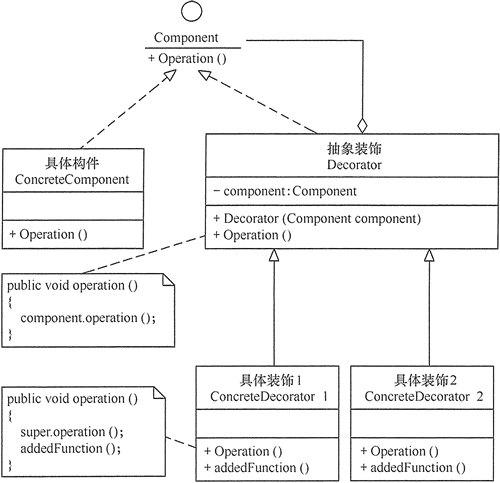
\includegraphics[width=0.8\textwidth]{image/12-1}
	\caption{装饰模式的结构图}
\end{figure}
\subsection{应用场景}
如Java的 Java I/O 标准库的设计:
\begin{lstlisting}
BufferedReader in=new BufferedReader(new FileReader("filename.txt));
String s=in.readLine();
\end{lstlisting}
\begin{enumerate}
	\item 当需要给一个现有类添加附加职责,而又不能采用生成子类的方法进行扩充时。例如,该类被隐藏或者该类是终极类或者采用继承方式会产生大量的子类。
	\item 当需要通过对现有的一组基本功能进行排列组合而产生非常多的功能时,采用继承关系很难实现,而采用装饰模式却很好实现。
	\item 当对象的功能要求可以动态地添加,也可以再动态地撤销时。
\end{enumerate}
\section{装饰模式的实现——例一}
\begin{table}[!h]
	\begin{tabular}{|l|l|}
		\hline
		名字&说明\\
		\hline
		Display&用于显示字符串的抽象类\\
		\hline
		StringDisplay&用于显示单行字符的类\\
		\hline
		Border&用于显示装饰边框的抽象类\\
		\hline
		SideBorder&用于只显示左右边框的类\\
		\hline
		FullBorder&用于显示上下左右边框的类\\
		\hline
		Main&测试类\\
		\hline
	\end{tabular}
\end{table}
\begin{lstlisting}
//可以显示多行字符串的抽象类
public abstract class Display {
	//获取横向字符数
	public abstract int getColumns();
	//获取纵向行数
	public abstract int getRows();
	//获取第 row 行的字符串
	public abstract String getRowText(int row);
	public final void show() {
		for (int i = 0; i < getRows(); i++) {
			System.out.println(getRowText(i));
		}
	}
}
\end{lstlisting}
\begin{lstlisting}
public class StringDispaly extends Display {
	private String string;
	public StringDispaly(String string) {
		this.string = string;
	}
	public int getColumns() {
		return string.getBytes().length;
	}
	public int getRows() {
		return 1;
	}
	public String getRowText(int row) {
		if (row == 0) {
			return string;
		} else {
			return null;
		}
	}
}
\end{lstlisting}
\begin{lstlisting}
/装饰边框的抽象类,装饰边框和被装饰物具有相同的方法
public abstract class Border extends Display {
	protected Display display;
	protected Border(Display display) {
		this.display = display;
	}
}
\end{lstlisting}
\begin{lstlisting}
//具体的装饰边框,装饰字符串的左右两侧
public class SideBorder extends Border {
	private char borderChar;
	public SideBorder(Display display, char borderChar) {
		super(display);
		this.borderChar = borderChar;
	}
	public int getColumns() {
		return 1 + display.getColumns() + 1;
	}
	public int getRows() {
		return display.getRows();
	}
	public String getRowText(int row) {
		return borderChar + display.getRowText(row) + borderChar;
	}
}
\end{lstlisting}
\begin{lstlisting}
//装饰字符串上下左右
public class FullBorder extends Border {
	public FullBorder(Display display) {
		super(display);
	}
	public int getColumns() {
		return 1 + display.getColumns() + 1;
	}
	public int getRows() {
		return 1 + display.getRows() + 1;
	}
	public String getRowText(int row) {
		if (row == 0) {
			return "+" + makeLine('-', display.getColumns()) + '+';
		} else if (row == display.getRows() + 1) {
			return "+" + makeLine('-', display.getColumns()) + '+';
		} else {
			return "|" + display.getRowText(row - 1) + '|';
		}
	}
	
	private String makeLine(char ch, int count) {
		StringBuffer buffer = new StringBuffer();
		for (int i = 0; i < count; i++) {
			buffer.append(ch);
		}
		return buffer.toString();
	}
}
\end{lstlisting}
\begin{lstlisting}
public class Main {
	public static void main(String[] args) {
		Display b1 = new StringDispaly("Hello, world.");
		Display b2 = new SideBorder(b1, '#');
		Display b3 = new FullBorder(b2);
		b1.show();
		b2.show();
		b3.show();
		Display b4 = new SideBorder(
			new FullBorder(
				new SideBorder(
					new FullBorder(
						new StringDispaly("Welcome, friend")
					), '*'
				)
			), '/'
		);
		b4.show();
	}
}
\end{lstlisting}
\begin{lstlisting}
//output
Hello, world.
#Hello, world.#
+---------------+
|#Hello, world.#|
+---------------+
/+-------------------+/
/|*+---------------+*|/
/|*|Welcome, friend|*|/
/|*+---------------+*|/
/+-------------------+/
\end{lstlisting}
\section{装饰模式实现——例二}
\begin{lstlisting}
//抽象构件角色
interface Component {
	public void operation();
}

//具体构件角色
class ConcreteComponent implements Component {
	public ConcreteComponent() {
		System.out.println("创建具体构件角色");
	}
	
	public void operation() {
		System.out.println("调用具体构件角色的方法operation()");
	}
}
\end{lstlisting}
\begin{lstlisting}
//抽象装饰角色
class Decorator implements Component {
	private Component component;
	public Decorator(Component component) {
		this.component = component;
	}
	public void operation() {
		component.operation();
	}
}

//具体装饰角色
class ConcreteDecorator extends Decorator {
	public ConcreteDecorator(Component component) {
		super(component);
	}
	
	public void operation() {
		super.operation();
		addedFunction();
	}
	
	public void addedFunction() {
		System.out.println("为具体构件角色增加额外的功能addedFunction()");
	}
}
\end{lstlisting}
\begin{lstlisting}
public class DecoratorPattern {
	public static void main(String[] args) {
		Component p = new ConcreteComponent();
		p.operation();
		System.out.println("---------------------------------");
		Component d = new ConcreteDecorator(p);
		d.operation();
	}
}
\end{lstlisting}
\begin{lstlisting}
//output
创建具体构件角色
调用具体构件角色的方法operation()
---------------------------------
调用具体构件角色的方法operation()
为具体构件角色增加额外的功能addedFunction()
\end{lstlisting}
\section{模式的扩展}
装饰模式所包含的 4 个角色不是任何时候都要存在的,在有些应用环境下模式是可以简化的。
\begin{enumerate}
	\item 如果只有一个具体构件而没有抽象构件时,可以让抽象装饰继承具体构件:
	\begin{figure}[!h]
		\centering
		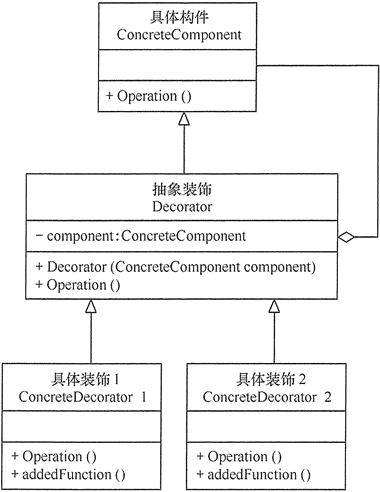
\includegraphics[width=0.5\textwidth]{image/12-2}
		\caption{只有一个具体构件的装饰模式}
	\end{figure}
	\item 如果只有一个具体装饰时,可以将抽象装饰和具体装饰合并:
	\begin{figure}[!h]
		\centering
		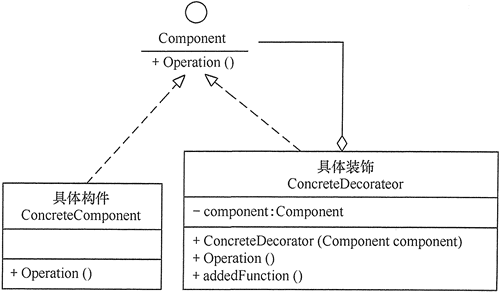
\includegraphics[width=0.5\textwidth]{image/12-3}
		\caption{只有一个具体装饰的装饰模式}
	\end{figure}
\end{enumerate}
\section{扩展思路}
\begin{enumerate}
	\item 接口的透明性:装饰边框和被装饰物具有一致性,装饰模式形成了类似于Composite的递归结构,
	但最内层还是与最外层一致,使用目的不同:装饰模式通过添加装饰物增加对象功能。
	\item 在不改变被装饰物的前提下增加功能,Decorator使用委托去递归处理;
	\item 可以动态地增加功能;
	\item 只需要一些装饰物就可以添加许多功能;
	\item java.io中大量使用装饰者模式;
	\item 导致增加很多小类。
\end{enumerate}
\section{相关设计模式}
\begin{enumerate}
	\item Adapter用于适配两个不同接口,Decorator可以在不改变被装饰物的前提下,为被装饰物添加边框(透明性);
	\item Strategy整体替换算法改变类型功能,Decorator可以像改变被装饰物的边框或是为被装饰物添加多重边框那样,增加类的功能。
\end{enumerate}
\section{延伸——继承和委托中的一致性}
\subsection{继承——父类和子类的一致性}
子类可以像操作父类方法一样操作子类的实例;
父类也可以通过类型转换操作子类。
\begin{lstlisting}
Parent obj = new Child();
obj.parentMethod();
(Child)obj.childMethod();
\end{lstlisting}
\subsection{委托——自已和被委托对象的一致性}
委托使得接口具有透明性,自已和被委托对象的一致性。
\begin{lstlisting}
interface Flower {
	void method();
}
class Rose implements Flower {
	Violet obj = ...
	void method () {
		obj.method();
	}
}
class Violet implements Flower {
	void method () {
		//...
	}
}
\end{lstlisting}